\documentclass[unicode]{beamer}

\usepackage[utf8]{inputenc}
\usepackage{cmap}
\usepackage[russian]{babel}

% listings
\usepackage{listings}
\lstset{language=java,frame=shadowbox,rulesepcolor=\color{gray},
        resetmargins=true,showstringspaces=false,
        basicstyle=\ttfamily,keywordstyle=\color{blue},
        stringstyle=\color{purple},commentstyle=\color{gray},
        morekeywords={assert,enum,@interface}}

% beamer
\usetheme{CambridgeUS}

\beamertemplatenavigationsymbolsempty

\setbeamertemplate{bibliography item}[book]
\setbeamertemplate{bibliography entry note}{//~}
\setbeamercolor{bibliography entry note}{fg=structure}


\title{Тестирование Java-программ}
\author{Алексей Владыкин}
\date{30 октября 2017}

\begin{document}

\begin{frame}
\titlepage
\end{frame}

\begin{frame}
\tableofcontents
\end{frame}


\section{Основные идеи}

\begin{frame}
\centering
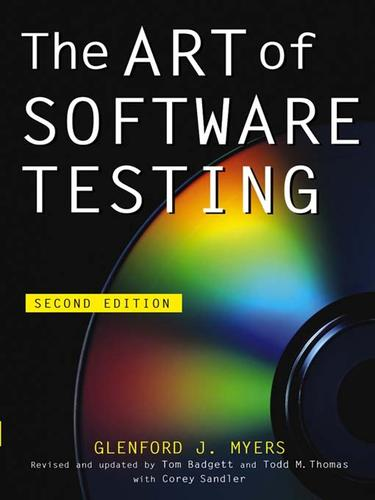
\includegraphics[width=0.4\textwidth]{pics/book.jpg}

Фундаментальная книга по тестированию
\end{frame}


\begin{frame}{Виды тестирования}
\begin{itemize}
\item \structure{Модульное тестирование} --- проверка работы
    программы на уровне отдельных модулей (классов, методов)
    \bigskip

\item \structure{Интеграционное тестирование} --- проверка
    совместной работы нескольких модулей
    \bigskip

\item \structure{Системное тестирование} --- проверка работы
    системы в целом
\end{itemize}
\end{frame}


\begin{frame}{Виды тестирования}
\begin{itemize}
\item Функциональное тестирование
    \bigskip

\item Тестирование производительности
    \bigskip

\item Тестирование удобства использования
    \bigskip

\item Тестирование безопасности
\end{itemize}
\end{frame}


\begin{frame}{Виды тестирования}
\begin{itemize}
\item Тестирование <<черного ящика>>
    \bigskip

\item Тестирование <<белого ящика>>
\end{itemize}
\end{frame}


\section{Модульное тестирование}


\begin{frame}
\centering
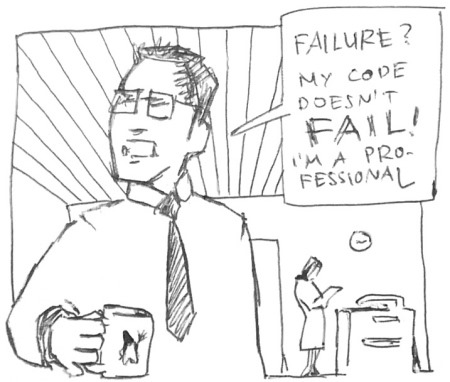
\includegraphics[width=0.7\textwidth]{pics/fail.jpg}
\end{frame}


\begin{frame}{Инструменты модульного тестирования}
\begin{itemize}
\item Инфраструктуры для написания и запуска тестов\\
    JUnit, TestNG
    \bigskip

\item Библиотеки проверок\\
    Hamcrest, AssertJ, XMLUnit, HttpUnit
    \bigskip

\item Библиотеки для создания тестовых дублеров\\
    Mockito, JMock, EasyMock
\end{itemize}
\end{frame}


\begin{frame}[fragile]{\texttt{assert}}
\begin{lstlisting}
assert "llo".equals("Hello".substring(3));

assert 1 == 1 : "Arithmetics broken";
\end{lstlisting}
\bigskip
\begin{itemize}
\item Поддерживаются только булевские условия
\item В исключении нет описания проблемы
\item Надо включать флагом JVM \texttt{-ea}
\end{itemize}
\end{frame}


\subsection{JUnit}


\begin{frame}[fragile]
\begin{itemize}
\item ``JUnit is a simple, open source framework
    to write and run repeatable tests.''
    \bigskip

\item \underline{\url{http://junit.org/}}
\bigskip
\begin{lstlisting}[language=xml,keywords={}]
<dependency>
    <groupId>org.junit.jupiter</groupId>
    <artifactId>junit-jupiter-api</artifactId>
    <version>5.0.1</version>
    <scope>test</scope>
</dependency>
\end{lstlisting}
\bigskip
\item \texttt{mvn test}
\end{itemize}
\end{frame}


\begin{frame}[fragile]
\begin{lstlisting}
package ru.csc.java.testing;

import org.junit.jupiter.api.Test;
import static org.junit.jupiter.api.Assertions.*;

public class AssertTest {

    @Test
    public void substring() {
        assertEquals("llo", "Hello".substring(3));
    }
}
\end{lstlisting}
\end{frame}


\begin{frame}[fragile]
\scriptsize
\begin{verbatim}
org.opentest4j.AssertionFailedError: 
Expected :llo
Actual   :lo
    at org.junit.jupiter.api.AssertionUtils.fail(AssertionUtils.java:52)
    at org.junit.jupiter.api.AssertEquals.failNotEqual(AssertEquals.java:177)
    at org.junit.jupiter.api.AssertEquals.assertEquals(AssertEquals.java:172)
    at org.junit.jupiter.api.AssertEquals.assertEquals(AssertEquals.java:163)
    at org.junit.jupiter.api.Assertions.assertEquals(Assertions.java:481)
    at ru.csc.java.testing.AssertTest.substring(AssertTest.java:11)
    ...
\end{verbatim}
\end{frame}


\begin{frame}{\texttt{org.junit.jupiter.api.Assertions}}
\begin{itemize}
\item \lstinline|assertTrue|\\
    \lstinline|assertFalse|
    \bigskip

\item \lstinline|assertEquals|\\
    \lstinline|assertArrayEquals|\\
    \lstinline|assertNotEquals|
    \bigskip

\item \lstinline|assertSame|\\
    \lstinline|assertNotSame|
    \bigskip

\item \lstinline|fail|
    \bigskip

\item Варианты с текстом ошибки и без
\end{itemize}
\end{frame}


\begin{frame}{Структура теста}
\begin{itemize}
\item (Given) Подготовка тестового окружения
    \bigskip

\item (When) Выполнение тестового сценария
    \bigskip

\item (Then) Проверки
\end{itemize}
\end{frame}


\begin{frame}{Жизненный цикл теста}
\begin{itemize}
\item \lstinline|@BeforeAll|
    \bigskip

\item Для каждого \lstinline|@Test|-метода:
    \begin{itemize}
    \item создание экземпляра тестового класса
    \item \lstinline|@BeforeEach|
    \item \lstinline|@Test|
    \item \lstinline|@AfterEach|
    \end{itemize}
    \bigskip

\item \lstinline|@AfterAll|
\end{itemize}
\end{frame}


\begin{frame}{Test Driven Development}
\begin{enumerate}
\item Пишем простейший тест, ломающий программу
    \bigskip

\item Пишем простейшую реализацию,\\ достаточную для прохождения теста
    \bigskip

\item Улучшаем написанный код, не ломая тесты.\\
    Возвращаемся к пункту~1
\end{enumerate}
\end{frame}


\subsection{Mockito}

\begin{frame}[fragile]
\begin{itemize}
\item ``Mockito is a mocking framework that tastes really good.''
    \bigskip

\item \underline{\url{https://code.google.com/p/mockito/}}
\end{itemize}
\bigskip
\begin{lstlisting}[language=xml,keywords={}]
<dependency>
    <groupId>org.mockito</groupId>
    <artifactId>mockito-core</artifactId>
    <version>2.11.0</version>
    <scope>test</scope>
</dependency>
\end{lstlisting}
\end{frame}



\section{Тестирование производительности}

\begin{frame}
\centering
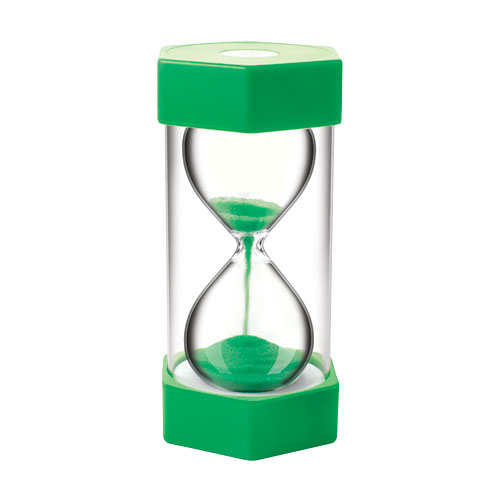
\includegraphics[width=0.7\textwidth]{pics/sandtimer.jpg}
\end{frame}


\subsection{JMH}

\begin{frame}
\begin{itemize}
\item ``JMH is a Java harness for building, running, and analysing
    nano/micro/milli/macro benchmarks written in Java and other
    languages targetting the JVM.''
    \bigskip
\item \underline{\url{http://openjdk.java.net/projects/code-tools/jmh/}}
\end{itemize}
\end{frame}


\end{document}

